%Clause Contingente 01 - jc
\begin{frame}
\begin{figure}[h!]
  \centering
  \begin{tikzpicture}[
      start chain=circle placed {at=(\tikzchaincount*-45+22.5+90:2.5)},
      lettre/.style={
        on chain,
        draw,
        circle,
        minimum size=1cm
      },
      chiffre/.style={
        node distance = 0.75cm
      },
      arr/.style={
        ->,
        >=triangle 90
      }
    ]
    \node[lettre] (1) {$\lnot x1$} ;
    \node[lettre] (5) {$x2$} ;
    \node[lettre] (3) {$\lnot x2$} ;
    \node[lettre] (6) {$x3$} ;
    \node[lettre] (4) {$\lnot x3$} ;
    \node[lettre] (7) {$x4$} ;
    \node[lettre] (2) {$\lnot x4$} ;
    \node[lettre] (8) {$x1$} ;

  \end{tikzpicture}
  \caption{Clause contingente : $(x_{1} \vee x_{2}) \wedge (x_{3} \vee x_{4})$}
  \label{fig:clause-conting}
\end{figure}
\end{frame}

%Clause Contingente 02 - jc
\begin{frame}
\begin{figure}[h!]
  \centering
  \begin{tikzpicture}[
      start chain=circle placed {at=(\tikzchaincount*-45+22.5+90:2.5)},
      lettre/.style={
        on chain,
        draw,
        circle,
        minimum size=1cm
      },
      chiffre/.style={
        node distance = 0.75cm
      },
      arr/.style={
        ->,
        >=triangle 90
      }
    ]
    \node[lettre] (1) {$\lnot x1$} ;
    \node[lettre] (5) {$x2$} ;
    \node[lettre] (3) {$\lnot x2$} ;
    \node[lettre] (6) {$x3$} ;
    \node[lettre] (4) {$\lnot x3$} ;
    \node[lettre] (7) {$x4$} ;
    \node[lettre] (2) {$\lnot x4$} ;
    \node[lettre] (8) {$x1$} ;
   

    \draw[arr] (1) -- (5) ;

  \end{tikzpicture}
  \caption{Clause contingente : $(x_{1} \vee x_{2}) \wedge (x_{3} \vee x_{4})$}
  \label{fig:clause-conting}
\end{figure}
\end{frame}

%Clause Contingente 03 - jc
\begin{frame}
\begin{figure}[h!]
  \centering
  \begin{tikzpicture}[
      start chain=circle placed {at=(\tikzchaincount*-45+22.5+90:2.5)},
      lettre/.style={
        on chain,
        draw,
        circle,
        minimum size=1cm
      },
      chiffre/.style={
        node distance = 0.75cm
      },
      arr/.style={
        ->,
        >=triangle 90
      }
    ]
    \node[lettre] (1) {$\lnot x1$} ;
    \node[lettre] (5) {$x2$} ;
    \node[lettre] (3) {$\lnot x2$} ;
    \node[lettre] (6) {$x3$} ;
    \node[lettre] (4) {$\lnot x3$} ;
    \node[lettre] (7) {$x4$} ;
    \node[lettre] (2) {$\lnot x4$} ;
    \node[lettre] (8) {$x1$} ;
   

    \draw[arr] (1) -- (5) ;
    \draw[arr] (3) -- (8) ;
  \end{tikzpicture}
  \caption{Clause contingente : $(x_{1} \vee x_{2}) \wedge (x_{3} \vee x_{4})$}
  \label{fig:clause-conting}
\end{figure}
\end{frame}

%Clause Contingente 04 - jc
\begin{frame}
\begin{figure}[h!]
  \centering
  \begin{tikzpicture}[
      start chain=circle placed {at=(\tikzchaincount*-45+22.5+90:2.5)},
      lettre/.style={
        on chain,
        draw,
        circle,
        minimum size=1cm
      },
      chiffre/.style={
        node distance = 0.75cm
      },
      arr/.style={
        ->,
        >=triangle 90
      }
    ]
    \node[lettre] (1) {$\lnot x1$} ;
    \node[lettre] (5) {$x2$} ;
    \node[lettre] (3) {$\lnot x2$} ;
    \node[lettre] (6) {$x3$} ;
    \node[lettre] (4) {$\lnot x3$} ;
    \node[lettre] (7) {$x4$} ;
    \node[lettre] (2) {$\lnot x4$} ;
    \node[lettre] (8) {$x1$} ;
   
    \draw[arr] (1) -- (5) ;
    \draw[arr] (3) -- (8) ;
    \draw[arr] (4) -- (7) ;
  \end{tikzpicture}
  \caption{Clause contingente : $(x_{1} \vee x_{2}) \wedge (x_{3} \vee x_{4})$}
  \label{fig:clause-conting}
\end{figure}
\end{frame}

%Clause Contingente 05 - jc
\begin{frame}
\begin{figure}[h!]
  \centering
  \begin{tikzpicture}[
      start chain=circle placed {at=(\tikzchaincount*-45+22.5+90:2.5)},
      lettre/.style={
        on chain,
        draw,
        circle,
        minimum size=1cm
      },
      chiffre/.style={
        node distance = 0.75cm
      },
      arr/.style={
        ->,
        >=triangle 90
      }
    ]
    \node[lettre] (1) {$\lnot x1$} ;
    \node[lettre] (5) {$x2$} ;
    \node[lettre] (3) {$\lnot x2$} ;
    \node[lettre] (6) {$x3$} ;
    \node[lettre] (4) {$\lnot x3$} ;
    \node[lettre] (7) {$x4$} ;
    \node[lettre] (2) {$\lnot x4$} ;
    \node[lettre] (8) {$x1$} ;
   
    \draw[arr] (1) -- (5) ;
    \draw[arr] (3) -- (8) ;
    \draw[arr] (2) -- (6) ;
    \draw[arr] (4) -- (7) ;
  \end{tikzpicture}
  \caption{Clause contingente : $(x_{1} \vee x_{2}) \wedge (x_{3} \vee x_{4})$}
  \label{fig:clause-conting}
\end{figure}
\end{frame}

%Clause Contingente 06 - jc
\begin{frame}
\begin{figure}[h!]
  \centering
  \begin{tikzpicture}[
      start chain=circle placed {at=(\tikzchaincount*-45+22.5+90:2.5)},
      lettre/.style={
        on chain,
        draw,
        circle,
        minimum size=1cm
      },
      chiffre/.style={
        node distance = 0.75cm
      },
      arr/.style={
        ->,
        >=triangle 90
      }
    ]
    \node[lettre] (1) {$\lnot x1$} ;
    \node[lettre] (5) {$x2$} ;
    \node[lettre] (3) {$\lnot x2$} ;
    \node[lettre] (6) {$x3$} ;
    \node[lettre] (4) {$\lnot x3$} ;
    \node[lettre] (7) {$x4$} ;
    \node[lettre] (2) {$\lnot x4$} ;
    \node[lettre] (8) {$x1$} ;
    
    \node[chiffre, above right of=1] {1} ;

    \draw[arr] (1) -- (5) ;
    \draw[arr] (3) -- (8) ;
    \draw[arr] (2) -- (6) ;
    \draw[arr] (4) -- (7) ;
  \end{tikzpicture}
  \caption{Clause contingente : $(x_{1} \vee x_{2}) \wedge (x_{3} \vee x_{4})$}
  \label{fig:clause-conting}
\end{figure}
\end{frame}

%Clause Contingente 07 - jc
\begin{frame}
\begin{figure}[h!]
  \centering
  \begin{tikzpicture}[
      start chain=circle placed {at=(\tikzchaincount*-45+22.5+90:2.5)},
      lettre/.style={
        on chain,
        draw,
        circle,
        minimum size=1cm
      },
      chiffre/.style={
        node distance = 0.75cm
      },
      arr/.style={
        ->,
        >=triangle 90
      }
    ]
    \node[lettre] (1) {$\lnot x1$} ;
    \node[lettre] (5) {$x2$} ;
    \node[lettre] (3) {$\lnot x2$} ;
    \node[lettre] (6) {$x3$} ;
    \node[lettre] (4) {$\lnot x3$} ;
    \node[lettre] (7) {$x4$} ;
    \node[lettre] (2) {$\lnot x4$} ;
    \node[lettre] (8) {$x1$} ;
    
    \node[chiffre, above right of=1] {1} ;
    \node[chiffre, above left of=2]  {2} ;

    \draw[arr] (1) -- (5) ;
    \draw[arr] (3) -- (8) ;
    \draw[arr] (2) -- (6) ;
    \draw[arr] (4) -- (7) ;
  \end{tikzpicture}
  \caption{Clause contingente : $(x_{1} \vee x_{2}) \wedge (x_{3} \vee x_{4})$}
  \label{fig:clause-conting}
\end{figure}
\end{frame}

%Clause Contingente 08 - jc
\begin{frame}
\begin{figure}[h!]
  \centering
  \begin{tikzpicture}[
      start chain=circle placed {at=(\tikzchaincount*-45+22.5+90:2.5)},
      lettre/.style={
        on chain,
        draw,
        circle,
        minimum size=1cm
      },
      chiffre/.style={
        node distance = 0.75cm
      },
      arr/.style={
        ->,
        >=triangle 90
      }
    ]
    \node[lettre] (1) {$\lnot x1$} ;
    \node[lettre] (5) {$x2$} ;
    \node[lettre] (3) {$\lnot x2$} ;
    \node[lettre] (6) {$x3$} ;
    \node[lettre] (4) {$\lnot x3$} ;
    \node[lettre] (7) {$x4$} ;
    \node[lettre] (2) {$\lnot x4$} ;
    \node[lettre] (8) {$x1$} ;
    
    \node[chiffre, above right of=1] {1} ;
    \node[chiffre, below right of=3] {3} ;
    \node[chiffre, above left of=2]  {2} ;

    \draw[arr] (1) -- (5) ;
    \draw[arr] (3) -- (8) ;
    \draw[arr] (2) -- (6) ;
    \draw[arr] (4) -- (7) ;
  \end{tikzpicture}
  \caption{Clause contingente : $(x_{1} \vee x_{2}) \wedge (x_{3} \vee x_{4})$}
  \label{fig:clause-conting}
\end{figure}
\end{frame}

%Clause Contingente 09 - jc
\begin{frame}
\begin{figure}[h!]
  \centering
  \begin{tikzpicture}[
      start chain=circle placed {at=(\tikzchaincount*-45+22.5+90:2.5)},
      lettre/.style={
        on chain,
        draw,
        circle,
        minimum size=1cm
      },
      chiffre/.style={
        node distance = 0.75cm
      },
      arr/.style={
        ->,
        >=triangle 90
      }
    ]
    \node[lettre] (1) {$\lnot x1$} ;
    \node[lettre] (5) {$x2$} ;
    \node[lettre] (3) {$\lnot x2$} ;
    \node[lettre] (6) {$x3$} ;
    \node[lettre] (4) {$\lnot x3$} ;
    \node[lettre] (7) {$x4$} ;
    \node[lettre] (2) {$\lnot x4$} ;
    \node[lettre] (8) {$x1$} ;
    
    \node[chiffre, above right of=1] {1} ;
    \node[chiffre, below right of=3] {3} ;
    \node[chiffre, below left of=4]  {4} ;
    \node[chiffre, above left of=2]  {2} ;

    \draw[arr] (1) -- (5) ;
    \draw[arr] (3) -- (8) ;
    \draw[arr] (2) -- (6) ;
    \draw[arr] (4) -- (7) ;
  \end{tikzpicture}
  \caption{Clause contingente : $(x_{1} \vee x_{2}) \wedge (x_{3} \vee x_{4})$}
  \label{fig:clause-conting}
\end{figure}
\end{frame}

%Clause Contingente 10 - jc
\begin{frame}
\begin{figure}[h!]
  \centering
  \begin{tikzpicture}[
      start chain=circle placed {at=(\tikzchaincount*-45+22.5+90:2.5)},
      lettre/.style={
        on chain,
        draw,
        circle,
        minimum size=1cm
      },
      chiffre/.style={
        node distance = 0.75cm
      },
      arr/.style={
        ->,
        >=triangle 90
      }
    ]
    \node[lettre] (1) {$\lnot x1$} ;
    \node[lettre] (5) {$x2$} ;
    \node[lettre] (3) {$\lnot x2$} ;
    \node[lettre] (6) {$x3$} ;
    \node[lettre] (4) {$\lnot x3$} ;
    \node[lettre] (7) {$x4$} ;
    \node[lettre] (2) {$\lnot x4$} ;
    \node[lettre] (8) {$x1$} ;
    
    \node[chiffre, above right of=1] {1} ;
    \node[chiffre, above right of=5] {5} ;
    \node[chiffre, below right of=3] {3} ;
    \node[chiffre, below left of=4]  {4} ;
    \node[chiffre, above left of=2]  {2} ;

    \draw[arr] (1) -- (5) ;
    \draw[arr] (3) -- (8) ;
    \draw[arr] (2) -- (6) ;
    \draw[arr] (4) -- (7) ;
  \end{tikzpicture}
  \caption{Clause contingente : $(x_{1} \vee x_{2}) \wedge (x_{3} \vee x_{4})$}
  \label{fig:clause-conting}
\end{figure}
\end{frame}

%Clause Contingente 11 - jc
\begin{frame}
\begin{figure}[h!]
  \centering
  \begin{tikzpicture}[
      start chain=circle placed {at=(\tikzchaincount*-45+22.5+90:2.5)},
      lettre/.style={
        on chain,
        draw,
        circle,
        minimum size=1cm
      },
      chiffre/.style={
        node distance = 0.75cm
      },
      arr/.style={
        ->,
        >=triangle 90
      }
    ]
    \node[lettre] (1) {$\lnot x1$} ;
    \node[lettre] (5) {$x2$} ;
    \node[lettre] (3) {$\lnot x2$} ;
    \node[lettre] (6) {$x3$} ;
    \node[lettre] (4) {$\lnot x3$} ;
    \node[lettre] (7) {$x4$} ;
    \node[lettre] (2) {$\lnot x4$} ;
    \node[lettre] (8) {$x1$} ;
    
    \node[chiffre, above right of=1] {1} ;
    \node[chiffre, above right of=5] {5} ;
    \node[chiffre, below right of=3] {3} ;
    \node[chiffre, below right of=6] {6} ;
    \node[chiffre, below left of=4]  {4} ;
    \node[chiffre, above left of=2]  {2} ;

    \draw[arr] (1) -- (5) ;
    \draw[arr] (3) -- (8) ;
    \draw[arr] (2) -- (6) ;
    \draw[arr] (4) -- (7) ;
  \end{tikzpicture}
  \caption{Clause contingente : $(x_{1} \vee x_{2}) \wedge (x_{3} \vee x_{4})$}
  \label{fig:clause-conting}
\end{figure}
\end{frame}

%Clause Contingente 12 - jc
\begin{frame}
\begin{figure}[h!]
  \centering
  \begin{tikzpicture}[
      start chain=circle placed {at=(\tikzchaincount*-45+22.5+90:2.5)},
      lettre/.style={
        on chain,
        draw,
        circle,
        minimum size=1cm
      },
      chiffre/.style={
        node distance = 0.75cm
      },
      arr/.style={
        ->,
        >=triangle 90
      }
    ]
    \node[lettre] (1) {$\lnot x1$} ;
    \node[lettre] (5) {$x2$} ;
    \node[lettre] (3) {$\lnot x2$} ;
    \node[lettre] (6) {$x3$} ;
    \node[lettre] (4) {$\lnot x3$} ;
    \node[lettre] (7) {$x4$} ;
    \node[lettre] (2) {$\lnot x4$} ;
    \node[lettre] (8) {$x1$} ;
    
    \node[chiffre, above right of=1] {1} ;
    \node[chiffre, above right of=5] {5} ;
    \node[chiffre, below right of=3] {3} ;
    \node[chiffre, below right of=6] {6} ;
    \node[chiffre, below left of=4]  {4} ;
    \node[chiffre, below left of=7]  {7} ;
    \node[chiffre, above left of=2]  {2} ;

    \draw[arr] (1) -- (5) ;
    \draw[arr] (3) -- (8) ;
    \draw[arr] (2) -- (6) ;
    \draw[arr] (4) -- (7) ;
  \end{tikzpicture}
  \caption{Clause contingente : $(x_{1} \vee x_{2}) \wedge (x_{3} \vee x_{4})$}
  \label{fig:clause-conting}
\end{figure}
\end{frame}

%Clause Contingente 13 - jc
\begin{frame}
\begin{figure}[h!]
  \centering
  \begin{tikzpicture}[
      start chain=circle placed {at=(\tikzchaincount*-45+22.5+90:2.5)},
      lettre/.style={
        on chain,
        draw,
        circle,
        minimum size=1cm
      },
      chiffre/.style={
        node distance = 0.75cm
      },
      arr/.style={
        ->,
        >=triangle 90
      }
    ]
    \node[lettre] (1) {$\lnot x1$} ;
    \node[lettre] (5) {$x2$} ;
    \node[lettre] (3) {$\lnot x2$} ;
    \node[lettre] (6) {$x3$} ;
    \node[lettre] (4) {$\lnot x3$} ;
    \node[lettre] (7) {$x4$} ;
    \node[lettre] (2) {$\lnot x4$} ;
    \node[lettre] (8) {$x1$} ;
    
    \node[chiffre, above right of=1] {1} ;
    \node[chiffre, above right of=5] {5} ;
    \node[chiffre, below right of=3] {3} ;
    \node[chiffre, below right of=6] {6} ;
    \node[chiffre, below left of=4]  {4} ;
    \node[chiffre, below left of=7]  {7} ;
    \node[chiffre, above left of=2]  {2} ;
    \node[chiffre, above left of=8]  {8} ;

    \draw[arr] (1) -- (5) ;
    \draw[arr] (3) -- (8) ;
    \draw[arr] (2) -- (6) ;
    \draw[arr] (4) -- (7) ;
  \end{tikzpicture}
  \caption{Clause contingente : $(x_{1} \vee x_{2}) \wedge (x_{3} \vee x_{4})$}
  \label{fig:clause-conting}
\end{figure}
\end{frame}

%Clause Contingente 14 - jc
\begin{frame}
\begin{figure}[h!]
  \centering
  \begin{tikzpicture}[
      start chain=circle placed {at=(\tikzchaincount*-45+22.5+90:2.5)},
      lettre/.style={
        on chain,
        draw,
        circle,
        minimum size=1cm
      },
      chiffre/.style={
        node distance = 0.75cm
      },
      arr/.style={
        ->,
        >=triangle 90
      }
    ]
    \node[lettre] (1) {$\lnot x1$} ;
    \node[lettre] (5) {$x2$} ;
    \node[lettre] (3) {$\lnot x2$} ;
    \node[lettre] (6) {$x3$} ;
    \node[lettre] (4) {$\lnot x3$} ;
    \node[lettre] (7) {$x4$} ;
    \node[lettre] (2) {$\lnot x4$} ;
    \node[lettre] (8) {$x1$} ;
    
    \node[left  of=8] {\textcolor{green!75!black}{vrai}} ;
    
    \node[chiffre, above right of=1] {1} ;
    \node[chiffre, above right of=5] {5} ;
    \node[chiffre, below right of=3] {3} ;
    \node[chiffre, below right of=6] {6} ;
    \node[chiffre, below left of=4]  {4} ;
    \node[chiffre, below left of=7]  {7} ;
    \node[chiffre, above left of=2]  {2} ;
    \node[chiffre, above left of=8]  {8} ;

    \draw[arr] (1) -- (5) ;
    \draw[arr] (3) -- (8) ;
    \draw[arr] (2) -- (6) ;
    \draw[arr] (4) -- (7) ;
  \end{tikzpicture}
  \caption{Clause contingente : $(x_{1} \vee x_{2}) \wedge (x_{3} \vee x_{4})$}
  \label{fig:clause-conting}
\end{figure}
\end{frame}

%Clause Contingente 15 - jc
\begin{frame}
\begin{figure}[h!]
  \centering
  \begin{tikzpicture}[
      start chain=circle placed {at=(\tikzchaincount*-45+22.5+90:2.5)},
      lettre/.style={
        on chain,
        draw,
        circle,
        minimum size=1cm
      },
      chiffre/.style={
        node distance = 0.75cm
      },
      arr/.style={
        ->,
        >=triangle 90
      }
    ]
    \node[lettre] (1) {$\lnot x1$} ;
    \node[lettre] (5) {$x2$} ;
    \node[lettre] (3) {$\lnot x2$} ;
    \node[lettre] (6) {$x3$} ;
    \node[lettre] (4) {$\lnot x3$} ;
    \node[lettre] (7) {$x4$} ;
    \node[lettre] (2) {$\lnot x4$} ;
    \node[lettre] (8) {$x1$} ;
    
    \node[right of=1] {\textcolor{red}{faux}} ;
    \node[left  of=8] {\textcolor{green!75!black}{vrai}} ;
    
    \node[chiffre, above right of=1] {1} ;
    \node[chiffre, above right of=5] {5} ;
    \node[chiffre, below right of=3] {3} ;
    \node[chiffre, below right of=6] {6} ;
    \node[chiffre, below left of=4]  {4} ;
    \node[chiffre, below left of=7]  {7} ;
    \node[chiffre, above left of=2]  {2} ;
    \node[chiffre, above left of=8]  {8} ;

    \draw[arr] (1) -- (5) ;
    \draw[arr] (3) -- (8) ;
    \draw[arr] (2) -- (6) ;
    \draw[arr] (4) -- (7) ;
  \end{tikzpicture}
  \caption{Clause contingente : $(x_{1} \vee x_{2}) \wedge (x_{3} \vee x_{4})$}
  \label{fig:clause-conting}
\end{figure}
\end{frame}

%Clause Contingente 16 - jc
\begin{frame}
\begin{figure}[h!]
  \centering
  \begin{tikzpicture}[
      start chain=circle placed {at=(\tikzchaincount*-45+22.5+90:2.5)},
      lettre/.style={
        on chain,
        draw,
        circle,
        minimum size=1cm
      },
      chiffre/.style={
        node distance = 0.75cm
      },
      arr/.style={
        ->,
        >=triangle 90
      }
    ]
    \node[lettre] (1) {$\lnot x1$} ;
    \node[lettre] (5) {$x2$} ;
    \node[lettre] (3) {$\lnot x2$} ;
    \node[lettre] (6) {$x3$} ;
    \node[lettre] (4) {$\lnot x3$} ;
    \node[lettre] (7) {$x4$} ;
    \node[lettre] (2) {$\lnot x4$} ;
    \node[lettre] (8) {$x1$} ;
    
    \node[right of=1] {\textcolor{red}{faux}} ;
    \node[left  of=7] {\textcolor{green!75!black}{vrai}} ;
    \node[left  of=8] {\textcolor{green!75!black}{vrai}} ;
    
    \node[chiffre, above right of=1] {1} ;
    \node[chiffre, above right of=5] {5} ;
    \node[chiffre, below right of=3] {3} ;
    \node[chiffre, below right of=6] {6} ;
    \node[chiffre, below left of=4]  {4} ;
    \node[chiffre, below left of=7]  {7} ;
    \node[chiffre, above left of=2]  {2} ;
    \node[chiffre, above left of=8]  {8} ;

    \draw[arr] (1) -- (5) ;
    \draw[arr] (3) -- (8) ;
    \draw[arr] (2) -- (6) ;
    \draw[arr] (4) -- (7) ;
  \end{tikzpicture}
  \caption{Clause contingente : $(x_{1} \vee x_{2}) \wedge (x_{3} \vee x_{4})$}
  \label{fig:clause-conting}
\end{figure}
\end{frame}

%Clause Contingente 17 - jc
\begin{frame}
\begin{figure}[h!]
  \centering
  \begin{tikzpicture}[
      start chain=circle placed {at=(\tikzchaincount*-45+22.5+90:2.5)},
      lettre/.style={
        on chain,
        draw,
        circle,
        minimum size=1cm
      },
      chiffre/.style={
        node distance = 0.75cm
      },
      arr/.style={
        ->,
        >=triangle 90
      }
    ]
    \node[lettre] (1) {$\lnot x1$} ;
    \node[lettre] (5) {$x2$} ;
    \node[lettre] (3) {$\lnot x2$} ;
    \node[lettre] (6) {$x3$} ;
    \node[lettre] (4) {$\lnot x3$} ;
    \node[lettre] (7) {$x4$} ;
    \node[lettre] (2) {$\lnot x4$} ;
    \node[lettre] (8) {$x1$} ;
    
    \node[right of=1] {\textcolor{red}{faux}} ;
    \node[left  of=7] {\textcolor{green!75!black}{vrai}} ;
    \node[left  of=2] {\textcolor{red}{faux}} ;
    \node[left  of=8] {\textcolor{green!75!black}{vrai}} ;
    
    \node[chiffre, above right of=1] {1} ;
    \node[chiffre, above right of=5] {5} ;
    \node[chiffre, below right of=3] {3} ;
    \node[chiffre, below right of=6] {6} ;
    \node[chiffre, below left of=4]  {4} ;
    \node[chiffre, below left of=7]  {7} ;
    \node[chiffre, above left of=2]  {2} ;
    \node[chiffre, above left of=8]  {8} ;

    \draw[arr] (1) -- (5) ;
    \draw[arr] (3) -- (8) ;
    \draw[arr] (2) -- (6) ;
    \draw[arr] (4) -- (7) ;
  \end{tikzpicture}
  \caption{Clause contingente : $(x_{1} \vee x_{2}) \wedge (x_{3} \vee x_{4})$}
  \label{fig:clause-conting}
\end{figure}
\end{frame}

%Clause Contingente 18 - jc
\begin{frame}
\begin{figure}[h!]
  \centering
  \begin{tikzpicture}[
      start chain=circle placed {at=(\tikzchaincount*-45+22.5+90:2.5)},
      lettre/.style={
        on chain,
        draw,
        circle,
        minimum size=1cm
      },
      chiffre/.style={
        node distance = 0.75cm
      },
      arr/.style={
        ->,
        >=triangle 90
      }
    ]
    \node[lettre] (1) {$\lnot x1$} ;
    \node[lettre] (5) {$x2$} ;
    \node[lettre] (3) {$\lnot x2$} ;
    \node[lettre] (6) {$x3$} ;
    \node[lettre] (4) {$\lnot x3$} ;
    \node[lettre] (7) {$x4$} ;
    \node[lettre] (2) {$\lnot x4$} ;
    \node[lettre] (8) {$x1$} ;
    
    \node[right of=1] {\textcolor{red}{faux}} ;
    \node[right of=6] {\textcolor{green!75!black}{vrai}} ;
    \node[left  of=7] {\textcolor{green!75!black}{vrai}} ;
    \node[left  of=2] {\textcolor{red}{faux}} ;
    \node[left  of=8] {\textcolor{green!75!black}{vrai}} ;
    
    \node[chiffre, above right of=1] {1} ;
    \node[chiffre, above right of=5] {5} ;
    \node[chiffre, below right of=3] {3} ;
    \node[chiffre, below right of=6] {6} ;
    \node[chiffre, below left of=4]  {4} ;
    \node[chiffre, below left of=7]  {7} ;
    \node[chiffre, above left of=2]  {2} ;
    \node[chiffre, above left of=8]  {8} ;

    \draw[arr] (1) -- (5) ;
    \draw[arr] (3) -- (8) ;
    \draw[arr] (2) -- (6) ;
    \draw[arr] (4) -- (7) ;
  \end{tikzpicture}
  \caption{Clause contingente : $(x_{1} \vee x_{2}) \wedge (x_{3} \vee x_{4})$}
  \label{fig:clause-conting}
\end{figure}
\end{frame}

%Clause Contingente 19 - jc
\begin{frame}
\begin{figure}[h!]
  \centering
  \begin{tikzpicture}[
      start chain=circle placed {at=(\tikzchaincount*-45+22.5+90:2.5)},
      lettre/.style={
        on chain,
        draw,
        circle,
        minimum size=1cm
      },
      chiffre/.style={
        node distance = 0.75cm
      },
      arr/.style={
        ->,
        >=triangle 90
      }
    ]
    \node[lettre] (1) {$\lnot x1$} ;
    \node[lettre] (5) {$x2$} ;
    \node[lettre] (3) {$\lnot x2$} ;
    \node[lettre] (6) {$x3$} ;
    \node[lettre] (4) {$\lnot x3$} ;
    \node[lettre] (7) {$x4$} ;
    \node[lettre] (2) {$\lnot x4$} ;
    \node[lettre] (8) {$x1$} ;
    
    \node[right of=1] {\textcolor{red}{faux}} ;
    \node[right of=6] {\textcolor{green!75!black}{vrai}} ;
    \node[left  of=4] {\textcolor{red}{faux}} ;
    \node[left  of=7] {\textcolor{green!75!black}{vrai}} ;
    \node[left  of=2] {\textcolor{red}{faux}} ;
    \node[left  of=8] {\textcolor{green!75!black}{vrai}} ;
    
    \node[chiffre, above right of=1] {1} ;
    \node[chiffre, above right of=5] {5} ;
    \node[chiffre, below right of=3] {3} ;
    \node[chiffre, below right of=6] {6} ;
    \node[chiffre, below left of=4]  {4} ;
    \node[chiffre, below left of=7]  {7} ;
    \node[chiffre, above left of=2]  {2} ;
    \node[chiffre, above left of=8]  {8} ;

    \draw[arr] (1) -- (5) ;
    \draw[arr] (3) -- (8) ;
    \draw[arr] (2) -- (6) ;
    \draw[arr] (4) -- (7) ;
  \end{tikzpicture}
  \caption{Clause contingente : $(x_{1} \vee x_{2}) \wedge (x_{3} \vee x_{4})$}
  \label{fig:clause-conting}
\end{figure}
\end{frame}

%Clause Contingente 20 - jc
\begin{frame}
\begin{figure}[h!]
  \centering
  \begin{tikzpicture}[
      start chain=circle placed {at=(\tikzchaincount*-45+22.5+90:2.5)},
      lettre/.style={
        on chain,
        draw,
        circle,
        minimum size=1cm
      },
      chiffre/.style={
        node distance = 0.75cm
      },
      arr/.style={
        ->,
        >=triangle 90
      }
    ]
    \node[lettre] (1) {$\lnot x1$} ;
    \node[lettre] (5) {$x2$} ;
    \node[lettre] (3) {$\lnot x2$} ;
    \node[lettre] (6) {$x3$} ;
    \node[lettre] (4) {$\lnot x3$} ;
    \node[lettre] (7) {$x4$} ;
    \node[lettre] (2) {$\lnot x4$} ;
    \node[lettre] (8) {$x1$} ;
    
    \node[right of=1] {\textcolor{red}{faux}} ;
    \node[right of=5] {\textcolor{green!75!black}{vrai}} ;
    \node[right of=6] {\textcolor{green!75!black}{vrai}} ;
    \node[left  of=4] {\textcolor{red}{faux}} ;
    \node[left  of=7] {\textcolor{green!75!black}{vrai}} ;
    \node[left  of=2] {\textcolor{red}{faux}} ;
    \node[left  of=8] {\textcolor{green!75!black}{vrai}} ;
    
    \node[chiffre, above right of=1] {1} ;
    \node[chiffre, above right of=5] {5} ;
    \node[chiffre, below right of=3] {3} ;
    \node[chiffre, below right of=6] {6} ;
    \node[chiffre, below left of=4]  {4} ;
    \node[chiffre, below left of=7]  {7} ;
    \node[chiffre, above left of=2]  {2} ;
    \node[chiffre, above left of=8]  {8} ;

    \draw[arr] (1) -- (5) ;
    \draw[arr] (3) -- (8) ;
    \draw[arr] (2) -- (6) ;
    \draw[arr] (4) -- (7) ;
  \end{tikzpicture}
  \caption{Clause contingente : $(x_{1} \vee x_{2}) \wedge (x_{3} \vee x_{4})$}
  \label{fig:clause-conting}
\end{figure}
\end{frame}

%Clause Contingente 21 - jc
\begin{frame}
\begin{figure}[h!]
  \centering
  \begin{tikzpicture}[
      start chain=circle placed {at=(\tikzchaincount*-45+22.5+90:2.5)},
      lettre/.style={
        on chain,
        draw,
        circle,
        minimum size=1cm
      },
      chiffre/.style={
        node distance = 0.75cm
      },
      arr/.style={
        ->,
        >=triangle 90
      }
    ]
    \node[lettre] (1) {$\lnot x1$} ;
    \node[lettre] (5) {$x2$} ;
    \node[lettre] (3) {$\lnot x2$} ;
    \node[lettre] (6) {$x3$} ;
    \node[lettre] (4) {$\lnot x3$} ;
    \node[lettre] (7) {$x4$} ;
    \node[lettre] (2) {$\lnot x4$} ;
    \node[lettre] (8) {$x1$} ;
    
    \node[right of=1] {\textcolor{red}{faux}} ;
    \node[right of=5] {\textcolor{green!75!black}{vrai}} ;
    \node[right of=3] {\textcolor{red}{faux}} ;
    \node[right of=6] {\textcolor{green!75!black}{vrai}} ;
    \node[left  of=4] {\textcolor{red}{faux}} ;
    \node[left  of=7] {\textcolor{green!75!black}{vrai}} ;
    \node[left  of=2] {\textcolor{red}{faux}} ;
    \node[left  of=8] {\textcolor{green!75!black}{vrai}} ;
    
    \node[chiffre, above right of=1] {1} ;
    \node[chiffre, above right of=5] {5} ;
    \node[chiffre, below right of=3] {3} ;
    \node[chiffre, below right of=6] {6} ;
    \node[chiffre, below left of=4]  {4} ;
    \node[chiffre, below left of=7]  {7} ;
    \node[chiffre, above left of=2]  {2} ;
    \node[chiffre, above left of=8]  {8} ;

    \draw[arr] (1) -- (5) ;
    \draw[arr] (3) -- (8) ;
    \draw[arr] (2) -- (6) ;
    \draw[arr] (4) -- (7) ;
  \end{tikzpicture}
  \caption{Clause contingente : $(x_{1} \vee x_{2}) \wedge (x_{3} \vee x_{4})$}
  \label{fig:clause-conting}
\end{figure}
\end{frame}

%Clause Valide 01 - jc
\begin{frame}
\begin{figure}[h!]
  \centering
  \begin{tikzpicture}[
      start chain=circle placed {at=(\tikzchaincount*-90+180:1.6)},
      lettre/.style={
        on chain,
        draw,
        circle,
        minimum size=1cm
      },
      chiffre/.style={
        node distance = 0.75cm
      },
      arr/.style={
        ->,
        >=triangle 90
      }
    ]
    \node[lettre] (1) {$\lnot x1$} ;
    \node[lettre] (2) {$x1$}  ;
    \node[lettre] (3) {$\lnot x2$} ;
    \node[lettre] (4) {$x2$}  ;

  \end{tikzpicture}
  \caption{Clause valide :  $(x_{1} \vee \neg x_{1}) \wedge (x_{2} \vee \neg x_{2})$}
  \label{fig:clause-valide}
\end{figure}
\end{frame}

%Clause Valide 02 - jc
\begin{frame}
\begin{figure}[h!]
  \centering
  \begin{tikzpicture}[
      start chain=circle placed {at=(\tikzchaincount*-90+180:1.6)},
      lettre/.style={
        on chain,
        draw,
        circle,
        minimum size=1cm
      },
      chiffre/.style={
        node distance = 0.75cm
      },
      arr/.style={
        ->,
        >=triangle 90
      }
    ]
    \node[lettre] (1) {$\lnot x1$} ;
    \node[lettre] (2) {$x1$}  ;
    \node[lettre] (3) {$\lnot x2$} ;
    \node[lettre] (4) {$x2$}  ;

	\path
       (1) edge[loop above] (1) ;
  \end{tikzpicture}
  \caption{Clause valide :  $(x_{1} \vee \neg x_{1}) \wedge (x_{2} \vee \neg x_{2})$}
  \label{fig:clause-valide}
\end{figure}
\end{frame}


%Clause Valide 03 - jc
\begin{frame}
\begin{figure}[h!]
  \centering
  \begin{tikzpicture}[
      start chain=circle placed {at=(\tikzchaincount*-90+180:1.6)},
      lettre/.style={
        on chain,
        draw,
        circle,
        minimum size=1cm
      },
      chiffre/.style={
        node distance = 0.75cm
      },
      arr/.style={
        ->,
        >=triangle 90
      }
    ]
    \node[lettre] (1) {$\lnot x1$} ;
    \node[lettre] (2) {$x1$}  ;
    \node[lettre] (3) {$\lnot x2$} ;
    \node[lettre] (4) {$x2$}  ;

	\path
       (1) edge[loop above] (1)
       (2) edge[loop above]  (2) ;
  \end{tikzpicture}
  \caption{Clause valide :  $(x_{1} \vee \neg x_{1}) \wedge (x_{2} \vee \neg x_{2})$}
  \label{fig:clause-valide}
\end{figure}
\end{frame}


%Clause Valide 04 - jc
\begin{frame}
\begin{figure}[h!]
  \centering
  \begin{tikzpicture}[
      start chain=circle placed {at=(\tikzchaincount*-90+180:1.6)},
      lettre/.style={
        on chain,
        draw,
        circle,
        minimum size=1cm
      },
      chiffre/.style={
        node distance = 0.75cm
      },
      arr/.style={
        ->,
        >=triangle 90
      }
    ]
    \node[lettre] (1) {$\lnot x1$} ;
    \node[lettre] (2) {$x1$}  ;
    \node[lettre] (3) {$\lnot x2$} ;
    \node[lettre] (4) {$x2$}  ;

	\path
       (1) edge[loop above] (1)
       (2) edge[loop above]  (2)
       (3) edge[loop below] (3) ;
  \end{tikzpicture}
  \caption{Clause valide :  $(x_{1} \vee \neg x_{1}) \wedge (x_{2} \vee \neg x_{2})$}
  \label{fig:clause-valide}
\end{figure}
\end{frame}


%Clause Valide 05 - jc
\begin{frame}
\begin{figure}[h!]
  \centering
  \begin{tikzpicture}[
      start chain=circle placed {at=(\tikzchaincount*-90+180:1.6)},
      lettre/.style={
        on chain,
        draw,
        circle,
        minimum size=1cm
      },
      chiffre/.style={
        node distance = 0.75cm
      },
      arr/.style={
        ->,
        >=triangle 90
      }
    ]
    \node[lettre] (1) {$\lnot x1$} ;
    \node[lettre] (2) {$x1$}  ;
    \node[lettre] (3) {$\lnot x2$} ;
    \node[lettre] (4) {$x2$}  ;

	\path
       (1) edge[loop above] (1)
       (2) edge[loop above]  (2)
       (3) edge[loop below] (3)
       (4) edge[loop above] (4) ;
  \end{tikzpicture}
  \caption{Clause valide :  $(x_{1} \vee \neg x_{1}) \wedge (x_{2} \vee \neg x_{2})$}
  \label{fig:clause-valide}
\end{figure}
\end{frame}


%Clause Valide 06 - jc
\begin{frame}
\begin{figure}[h!]
  \centering
  \begin{tikzpicture}[
      start chain=circle placed {at=(\tikzchaincount*-90+180:1.6)},
      lettre/.style={
        on chain,
        draw,
        circle,
        minimum size=1cm
      },
      chiffre/.style={
        node distance = 0.75cm
      },
      arr/.style={
        ->,
        >=triangle 90
      }
    ]
    \node[lettre] (1) {$\lnot x1$} ;
    \node[lettre] (2) {$x1$}  ;
    \node[lettre] (3) {$\lnot x2$} ;
    \node[lettre] (4) {$x2$}  ;
    
    \node[chiffre, above right of=1] {1} ;

	\path
       (1) edge[loop above] (1)
       (2) edge[loop above]  (2)
       (3) edge[loop below] (3)
       (4) edge[loop above] (4) ;
  \end{tikzpicture}
  \caption{Clause valide :  $(x_{1} \vee \neg x_{1}) \wedge (x_{2} \vee \neg x_{2})$}
  \label{fig:clause-valide}
\end{figure}
\end{frame}


%Clause Valide 07 - jc
\begin{frame}
\begin{figure}[h!]
  \centering
  \begin{tikzpicture}[
      start chain=circle placed {at=(\tikzchaincount*-90+180:1.6)},
      lettre/.style={
        on chain,
        draw,
        circle,
        minimum size=1cm
      },
      chiffre/.style={
        node distance = 0.75cm
      },
      arr/.style={
        ->,
        >=triangle 90
      }
    ]
    \node[lettre] (1) {$\lnot x1$} ;
    \node[lettre] (2) {$x1$}  ;
    \node[lettre] (3) {$\lnot x2$} ;
    \node[lettre] (4) {$x2$}  ;
    
    \node[chiffre, above right of=1] {1} ;
    \node[chiffre, below right of=2] {2} ;

	\path
       (1) edge[loop above] (1)
       (2) edge[loop above]  (2)
       (3) edge[loop below] (3)
       (4) edge[loop above] (4) ;
  \end{tikzpicture}
  \caption{Clause valide :  $(x_{1} \vee \neg x_{1}) \wedge (x_{2} \vee \neg x_{2})$}
  \label{fig:clause-valide}
\end{figure}
\end{frame}




%Clause Valide 08 - jc
\begin{frame}
\begin{figure}[h!]
  \centering
  \begin{tikzpicture}[
      start chain=circle placed {at=(\tikzchaincount*-90+180:1.6)},
      lettre/.style={
        on chain,
        draw,
        circle,
        minimum size=1cm
      },
      chiffre/.style={
        node distance = 0.75cm
      },
      arr/.style={
        ->,
        >=triangle 90
      }
    ]
    \node[lettre] (1) {$\lnot x1$} ;
    \node[lettre] (2) {$x1$}  ;
    \node[lettre] (3) {$\lnot x2$} ;
    \node[lettre] (4) {$x2$}  ;
    
    \node[chiffre, above right of=1] {1} ;
    \node[chiffre, below right of=2] {2} ;
    \node[chiffre, below right of=3]  {3} ;

	\path
       (1) edge[loop above] (1)
       (2) edge[loop above]  (2)
       (3) edge[loop below] (3)
       (4) edge[loop above] (4) ;
  \end{tikzpicture}
  \caption{Clause valide :  $(x_{1} \vee \neg x_{1}) \wedge (x_{2} \vee \neg x_{2})$}
  \label{fig:clause-valide}
\end{figure}
\end{frame}

%Clause Valide 09 - jc
\begin{frame}
\begin{figure}[h!]
  \centering
  \begin{tikzpicture}[
      start chain=circle placed {at=(\tikzchaincount*-90+180:1.6)},
      lettre/.style={
        on chain,
        draw,
        circle,
        minimum size=1cm
      },
      chiffre/.style={
        node distance = 0.75cm
      },
      arr/.style={
        ->,
        >=triangle 90
      }
    ]
    \node[lettre] (1) {$\lnot x1$} ;
    \node[lettre] (2) {$x1$}  ;
    \node[lettre] (3) {$\lnot x2$} ;
    \node[lettre] (4) {$x2$}  ;
    
    \node[chiffre, above right of=1] {1} ;
    \node[chiffre, below right of=2] {2} ;
    \node[chiffre, below right of=3]  {3} ;
    \node[chiffre, below left of=4]  {4} ;

	\path
       (1) edge[loop above] (1)
       (2) edge[loop above]  (2)
       (3) edge[loop below] (3)
       (4) edge[loop above] (4) ;
  \end{tikzpicture}
  \caption{Clause valide :  $(x_{1} \vee \neg x_{1}) \wedge (x_{2} \vee \neg x_{2})$}
  \label{fig:clause-valide}
\end{figure}
\end{frame}


%Clause Valide 10 - jc
\begin{frame}
\begin{figure}[h!]
  \centering
  \begin{tikzpicture}[
      start chain=circle placed {at=(\tikzchaincount*-90+180:1.6)},
      lettre/.style={
        on chain,
        draw,
        circle,
        minimum size=1cm
      },
      chiffre/.style={
        node distance = 0.75cm
      },
      arr/.style={
        ->,
        >=triangle 90
      }
    ]
    \node[lettre] (1) {$\lnot x1$} ;
    \node[lettre] (2) {$x1$}  ;
    \node[lettre] (3) {$\lnot x2$} ;
    \node[lettre] (4) {$x2$}  ;
    
    \node[left  of=4] {\textcolor{green!75!black}{vrai}} ;
    
    \node[chiffre, above right of=1] {1} ;
    \node[chiffre, below right of=2] {2} ;
    \node[chiffre, below right of=3]  {3} ;
    \node[chiffre, below left of=4]  {4} ;

	\path
       (1) edge[loop above] (1)
       (2) edge[loop above]  (2)
       (3) edge[loop below] (3)
       (4) edge[loop above] (4) ;
  \end{tikzpicture}
  \caption{Clause valide :  $(x_{1} \vee \neg x_{1}) \wedge (x_{2} \vee \neg x_{2})$}
  \label{fig:clause-valide}
\end{figure}
\end{frame}


%Clause Valide 11 - jc
\begin{frame}
\begin{figure}[h!]
  \centering
  \begin{tikzpicture}[
      start chain=circle placed {at=(\tikzchaincount*-90+180:1.6)},
      lettre/.style={
        on chain,
        draw,
        circle,
        minimum size=1cm
      },
      chiffre/.style={
        node distance = 0.75cm
      },
      arr/.style={
        ->,
        >=triangle 90
      }
    ]
    \node[lettre] (1) {$\lnot x1$} ;
    \node[lettre] (2) {$x1$}  ;
    \node[lettre] (3) {$\lnot x2$} ;
    \node[lettre] (4) {$x2$}  ;
   
    \node[right of=3] {\textcolor{red}{faux}} ;
    \node[left  of=4] {\textcolor{green!75!black}{vrai}} ;
    
    \node[chiffre, above right of=1] {1} ;
    \node[chiffre, below right of=2] {2} ;
    \node[chiffre, below right of=3]  {3} ;
    \node[chiffre, below left of=4]  {4} ;

	\path
       (1) edge[loop above] (1)
       (2) edge[loop above]  (2)
       (3) edge[loop below] (3)
       (4) edge[loop above] (4) ;
  \end{tikzpicture}
  \caption{Clause valide :  $(x_{1} \vee \neg x_{1}) \wedge (x_{2} \vee \neg x_{2})$}
  \label{fig:clause-valide}
\end{figure}
\end{frame}


%Clause Valide 12 - jc
\begin{frame}
\begin{figure}[h!]
  \centering
  \begin{tikzpicture}[
      start chain=circle placed {at=(\tikzchaincount*-90+180:1.6)},
      lettre/.style={
        on chain,
        draw,
        circle,
        minimum size=1cm
      },
      chiffre/.style={
        node distance = 0.75cm
      },
      arr/.style={
        ->,
        >=triangle 90
      }
    ]
    \node[lettre] (1) {$\lnot x1$} ;
    \node[lettre] (2) {$x1$}  ;
    \node[lettre] (3) {$\lnot x2$} ;
    \node[lettre] (4) {$x2$}  ;
    
    \node[right of=2] {\textcolor{green!75!black}{vrai}};
    \node[right of=3] {\textcolor{red}{faux}} ;
    \node[left  of=4] {\textcolor{green!75!black}{vrai}} ;
    
    \node[chiffre, above right of=1] {1} ;
    \node[chiffre, below right of=2] {2} ;
    \node[chiffre, below right of=3]  {3} ;
    \node[chiffre, below left of=4]  {4} ;

	\path
       (1) edge[loop above] (1)
       (2) edge[loop above]  (2)
       (3) edge[loop below] (3)
       (4) edge[loop above] (4) ;
  \end{tikzpicture}
  \caption{Clause valide :  $(x_{1} \vee \neg x_{1}) \wedge (x_{2} \vee \neg x_{2})$}
  \label{fig:clause-valide}
\end{figure}
\end{frame}


%Clause Valide 13 - jc
\begin{frame}
\begin{figure}[h!]
  \centering
  \begin{tikzpicture}[
      start chain=circle placed {at=(\tikzchaincount*-90+180:1.6)},
      lettre/.style={
        on chain,
        draw,
        circle,
        minimum size=1cm
      },
      chiffre/.style={
        node distance = 0.75cm
      },
      arr/.style={
        ->,
        >=triangle 90
      }
    ]
    \node[lettre] (1) {$\lnot x1$} ;
    \node[lettre] (2) {$x1$}  ;
    \node[lettre] (3) {$\lnot x2$} ;
    \node[lettre] (4) {$x2$}  ;
    
    \node[right of=1] {\textcolor{red}{faux}}  ;
    \node[right of=2] {\textcolor{green!75!black}{vrai}};
    \node[right of=3] {\textcolor{red}{faux}} ;
    \node[left  of=4] {\textcolor{green!75!black}{vrai}} ;
    
    \node[chiffre, above right of=1] {1} ;
    \node[chiffre, below right of=2] {2} ;
    \node[chiffre, below right of=3]  {3} ;
    \node[chiffre, below left of=4]  {4} ;

	\path
       (1) edge[loop above] (1)
       (2) edge[loop above]  (2)
       (3) edge[loop below] (3)
       (4) edge[loop above] (4) ;
  \end{tikzpicture}
  \caption{Clause valide :  $(x_{1} \vee \neg x_{1}) \wedge (x_{2} \vee \neg x_{2})$}
  \label{fig:clause-valide}
\end{figure}
\end{frame}

% clause insatisfiable 01 - jc
\begin{frame}
\begin{figure}[h!]
  \centering
  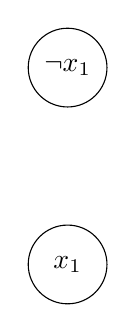
\begin{tikzpicture}[
      node distance=2.5cm,
      lettre/.style={
        draw,
        circle,
        minimum size=1cm
      }
    ]
    \node[lettre] (nx1) {$\lnot x_1$} ;
    \node[lettre, below of=nx1] (x1) {$x_1$} ;
    \node[coordinate,xshift=0.1cm] (x1r) at (x1.north) {};
    \node[coordinate,xshift=-0.1cm] (x1l) at (x1.north) {};
    \node[coordinate,xshift=0.1cm] (nx1r) at (nx1.south) {};
    \node[coordinate,xshift=-0.1cm] (nx1l) at (nx1.south) {};

  \end{tikzpicture}
  \caption{Clause insatisfiable : $(x_{1} \vee x_{1}) \wedge (\neg x_{1} \vee \neg x_{1})$}
  \label{fig:clause-insat}
\end{figure}
\end{frame}

% clause insatisfiable 02 - jc
\begin{frame}
\begin{figure}[h!]
  \centering
  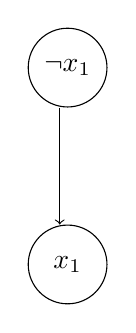
\begin{tikzpicture}[
      node distance=2.5cm,
      lettre/.style={
        draw,
        circle,
        minimum size=1cm
      }
    ]
    \node[lettre] (nx1) {$\lnot x_1$} ;
    \node[lettre, below of=nx1] (x1) {$x_1$} ;
    \node[coordinate,xshift=0.1cm] (x1r) at (x1.north) {};
    \node[coordinate,xshift=-0.1cm] (x1l) at (x1.north) {};
    \node[coordinate,xshift=0.1cm] (nx1r) at (nx1.south) {};
    \node[coordinate,xshift=-0.1cm] (nx1l) at (nx1.south) {};
    \draw[->] (nx1l) -- (x1l);

  \end{tikzpicture}
  \caption{Clause insatisfiable : $(x_{1} \vee x_{1}) \wedge (\neg x_{1} \vee \neg x_{1})$}
  \label{fig:clause-insat}
\end{figure}
\end{frame}

% clause insatisfiable 03 - jc
\begin{frame}
\begin{figure}[h!]
  \centering
  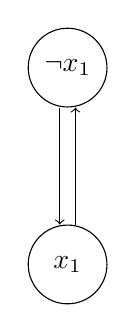
\begin{tikzpicture}[
      node distance=2.5cm,
      lettre/.style={
        draw,
        circle,
        minimum size=1cm
      }
    ]
    \node[lettre] (nx1) {$\lnot x_1$} ;
    \node[lettre, below of=nx1] (x1) {$x_1$} ;
    \node[coordinate,xshift=0.1cm] (x1r) at (x1.north) {};
    \node[coordinate,xshift=-0.1cm] (x1l) at (x1.north) {};
    \node[coordinate,xshift=0.1cm] (nx1r) at (nx1.south) {};
    \node[coordinate,xshift=-0.1cm] (nx1l) at (nx1.south) {};
    \draw[->] (x1r) -- (nx1r);
    \draw[->] (nx1l) -- (x1l);
  \end{tikzpicture}
  \caption{Clause insatisfiable : $(x_{1} \vee x_{1}) \wedge (\neg x_{1} \vee \neg x_{1})$}
  \label{fig:clause-insat}
\end{figure}
\end{frame}

% clause insatisfiable 04 - jc
\begin{frame}
\begin{figure}[h!]
  \centering
  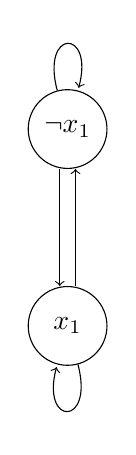
\begin{tikzpicture}[
      node distance=2.5cm,
      lettre/.style={
        draw,
        circle,
        minimum size=1cm
      }
    ]
    \node[lettre] (nx1) {$\lnot x_1$} ;
    \node[lettre, below of=nx1] (x1) {$x_1$} ;
    \node[coordinate,xshift=0.1cm] (x1r) at (x1.north) {};
    \node[coordinate,xshift=-0.1cm] (x1l) at (x1.north) {};
    \node[coordinate,xshift=0.1cm] (nx1r) at (nx1.south) {};
    \node[coordinate,xshift=-0.1cm] (nx1l) at (nx1.south) {};
    \draw[->] (x1r) -- (nx1r);
    \draw[->] (nx1l) -- (x1l);
    \path
      (x1) edge[loop below] (x1)
      (nx1) edge[loop above] (nx1) ;
  \end{tikzpicture}
  \caption{Clause insatisfiable : $(x_{1} \vee x_{1}) \wedge (\neg x_{1} \vee \neg x_{1})$}
  \label{fig:clause-insat}
\end{figure}
\end{frame}
